\chapter{Experimental Setup}
\label{chap:exp}
The accelerators are utilized to recreate the high energy environment rich in new physics like the hot early universe. In this thesis, Large Hadron Collider (LHC) is used for this purpose, and the ATLAS detector (A Toroidal LHC ApparatuS) is taken to probe the potential signatures of new physics. 
\section{Large Hadron Collider }
LHC is a circular collider with diameter of 27km for hadrons (it could be either proton or lead ion) hosted by CERN at the border of France and Switzerland in the depth varied between 50m to 175m. It accelerates protons (lead ions) to the speed of Lorentz Factor of 10540 (32) and smashes them together to recreate the ``hot'' environment right after the big bang which corresponds to 6.5TeV (2.5TeV) energy. However, before a proton reaches the targeted energy, it has a long way to go.
\\
\\{\bf Ionization}
\\
\\At the beginning, hydrogen is released from a tank and ionized into the state of proton-electron plasma. It then experiences the electric field to separate electrons as well as protons like Fig. \ref{Fig:ionization}. The protons are then taken out and sent into the LINAC2, a linear accelerator. After reaching the energy of $450MeV$, the protons are fed into circular accelerators in the order of the PSB, PS and SPS to further increase the energy until they reach 450$GeV$ (Fig. \ref{Fig:boost}). By this stage, the protons are ready to be injected into the LHC.
\begin{figure}[!h]                
	\includegraphics[width=0.25\textwidth]{Chapter2/ionization.png}
	\centering
	\begin{center}
		\caption{The hydrogen plasma is separated into electrons (red) and protons (blue)}
		\label{Fig:ionization}            
	\end{center}
\end{figure}
\\
\begin{figure}[!h]                
	\includegraphics[width=0.86\textwidth]{Chapter2/pre-acceleration.jpg}
	\centering
	\begin{center}
		\caption{Before the LHC, protons go through several boosting facilities}
		\label{Fig:boost}            
	\end{center}
\end{figure}
{\bf Magnets}
\\
\\While accelerating the protons, they  would repel each other due to the same electric charge they are carrying, so the quadrupole magnets are implemented in LHC to focus them by the effect of magnetic lens. In addition to the quadrupole magnets, the other magnet system in LHC is the superconducting dipole magnets working to bend the protons to keep them staying in the circular pipe of the LHC. The dipole system was upgraded between 2012 and 2015 to provide a 8.3T magnetic field to bend the proton beam at an energy of 6.5TeV.
\\
\\{\bf Radiofrequency Cavity}  
\\
\\The ``radiofrequency cavity'' (RF cavity) is in charge of the acceleration. Protons would experience electric field when going through RF cavities which are installed in the LHC like beads along a string. The field is induced by an alternating current of a frequency of $400~MHz$ and resonates as a standing wave in the cavity. This wave decelerates faster protons and accelerates slower ones, which makes the protons squeeze into bunches as demonstrated in Fig. \ref{Fig:bunch}., until they reach the targeted energy. When the beams are kept in the same speed, they are called ``stable beams'' and ready for the collision. 
\begin{figure}[!h]                
	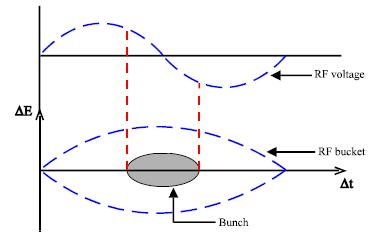
\includegraphics[width=0.3\textwidth]{Chapter2/bunch.png}
	\centering
	\begin{center}
		\caption{The protons are formed into a bunch in the EM wave}
		\label{Fig:bunch}            
	\end{center}
\end{figure}
Each LHC beam could have up to 3564 bunches with $\mathcal{O}^{12}$ protons in each bunch for a spacing of 25ns, but not all of them are filled. For the LHC 2018 operation, the ``filling scheme''  has around 1000-2500 bunches filled, while the remaining ones are left empty (filling scheme most of time is constrained due to technical issues). A series of continuous bunches is called a ``bunch train''. This scheme would then be used to configure the trigger and data acquisition system for the active window of detector operation.
\\  
\\{\bf Collision}
\\
\\The LHC has two beams going in opposite directions with the same configuration (bunch structure, luminosity and energy), and the two beams cross at locations where four detectors are sited: ALICE, ATLAS, CMS, and LHCb. Before stable beams, the two beams pass each other where they are supposed to cross. When both of the beams are ready, the two beams are slightly shifted to target on each other for the collisions .  The crossing angle between the two beams plays an important role in detector performance. It should not be too big, or it would have an impact on physical object reconstruction (see section. \ref{sec:obj rec}) which assumed a zero crossing angle. However, it also should not be too small, or the two beams would interfere with each other. The crossing angle is kept optimized during LHC operation even when the detectors are taking data for physics.
\\
\\When collisions happen, the two crossed bunches usually have more than one pair of interacting protons. In physics, only the most energetic one gets the attention for study, while the other ones are the background contribution called "pile-up events". For ATLAS 2018 operation, the pile-up events could number up to 70 per bunch crossing, and it is now a major challenge of analyses to suppress this type of background.  
\section{ATLAS Detector}
The ATLAS detector (A Toroidal LHC ApparatuS) is designed as a general purpose detector\footnote{The other general purpose detector hosted by LHC is Compact Muon Solenoid (CMS). The discovery of any new physics shall be verified by both the ATLAS and CMS collaborations} aiming for most high energy physics physics topics in the energy scale LHC provides like SM precision measurement and searches for new physics.

The ATLAS detector is in a cylinder shape with dimensions of 44m in length and 25m in diameter. Its inner structure is like an onion with multiple layers from the inner most tracking system to the outer part of muon spectrometer functioning to capture different physical objects which will be explained in the following. In the purpose of measuring the particle mass and charge, ATLAS also has two magnetic systems (a solenoid and a toroid) located outside inner tracking system and muon spectrometer. The diagram of the whole ATLAS detector is shown in Fig. \ref{Fig:ATLAS}.

\begin{figure}[!h]                
	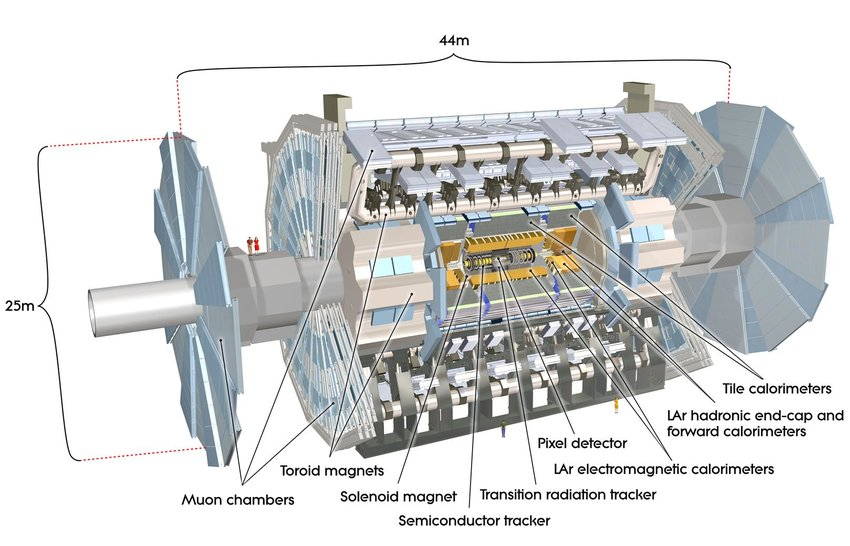
\includegraphics[width=0.8\textwidth]{Chapter2/ATLAS.jpg}
	\centering
	\begin{center}
		\caption{The diagram of the ATLAS detector}
		\label{Fig:ATLAS}            
	\end{center}
\end{figure}

To define the object positions inside this massive and complicated giant, the coordinate is applied as shown in Fig. \ref{Fig:coordinate}. The x-axis is defined pointing to the centre of the LHC, while the z-axis is the cylinder axle toward the direction of solenoid magnetic field. Then, the y-axis could be found with the right-hand rule. However, this Cartesian coordinate is not convenient in a cylinder, so, instead, the spherical system ($\theta$:angle related to z-axis, $\phi$:angle related to x-axis) is adopted in terms of physics. To keep the parameters as Lorentz invariance, $\theta$ is interpreted into pseudorapidity, $\eta$:
\begin{equation}
\eta = -\ln{\tan{\frac{\theta}{2}}}
\end{equation}
\begin{figure}[!h]                
	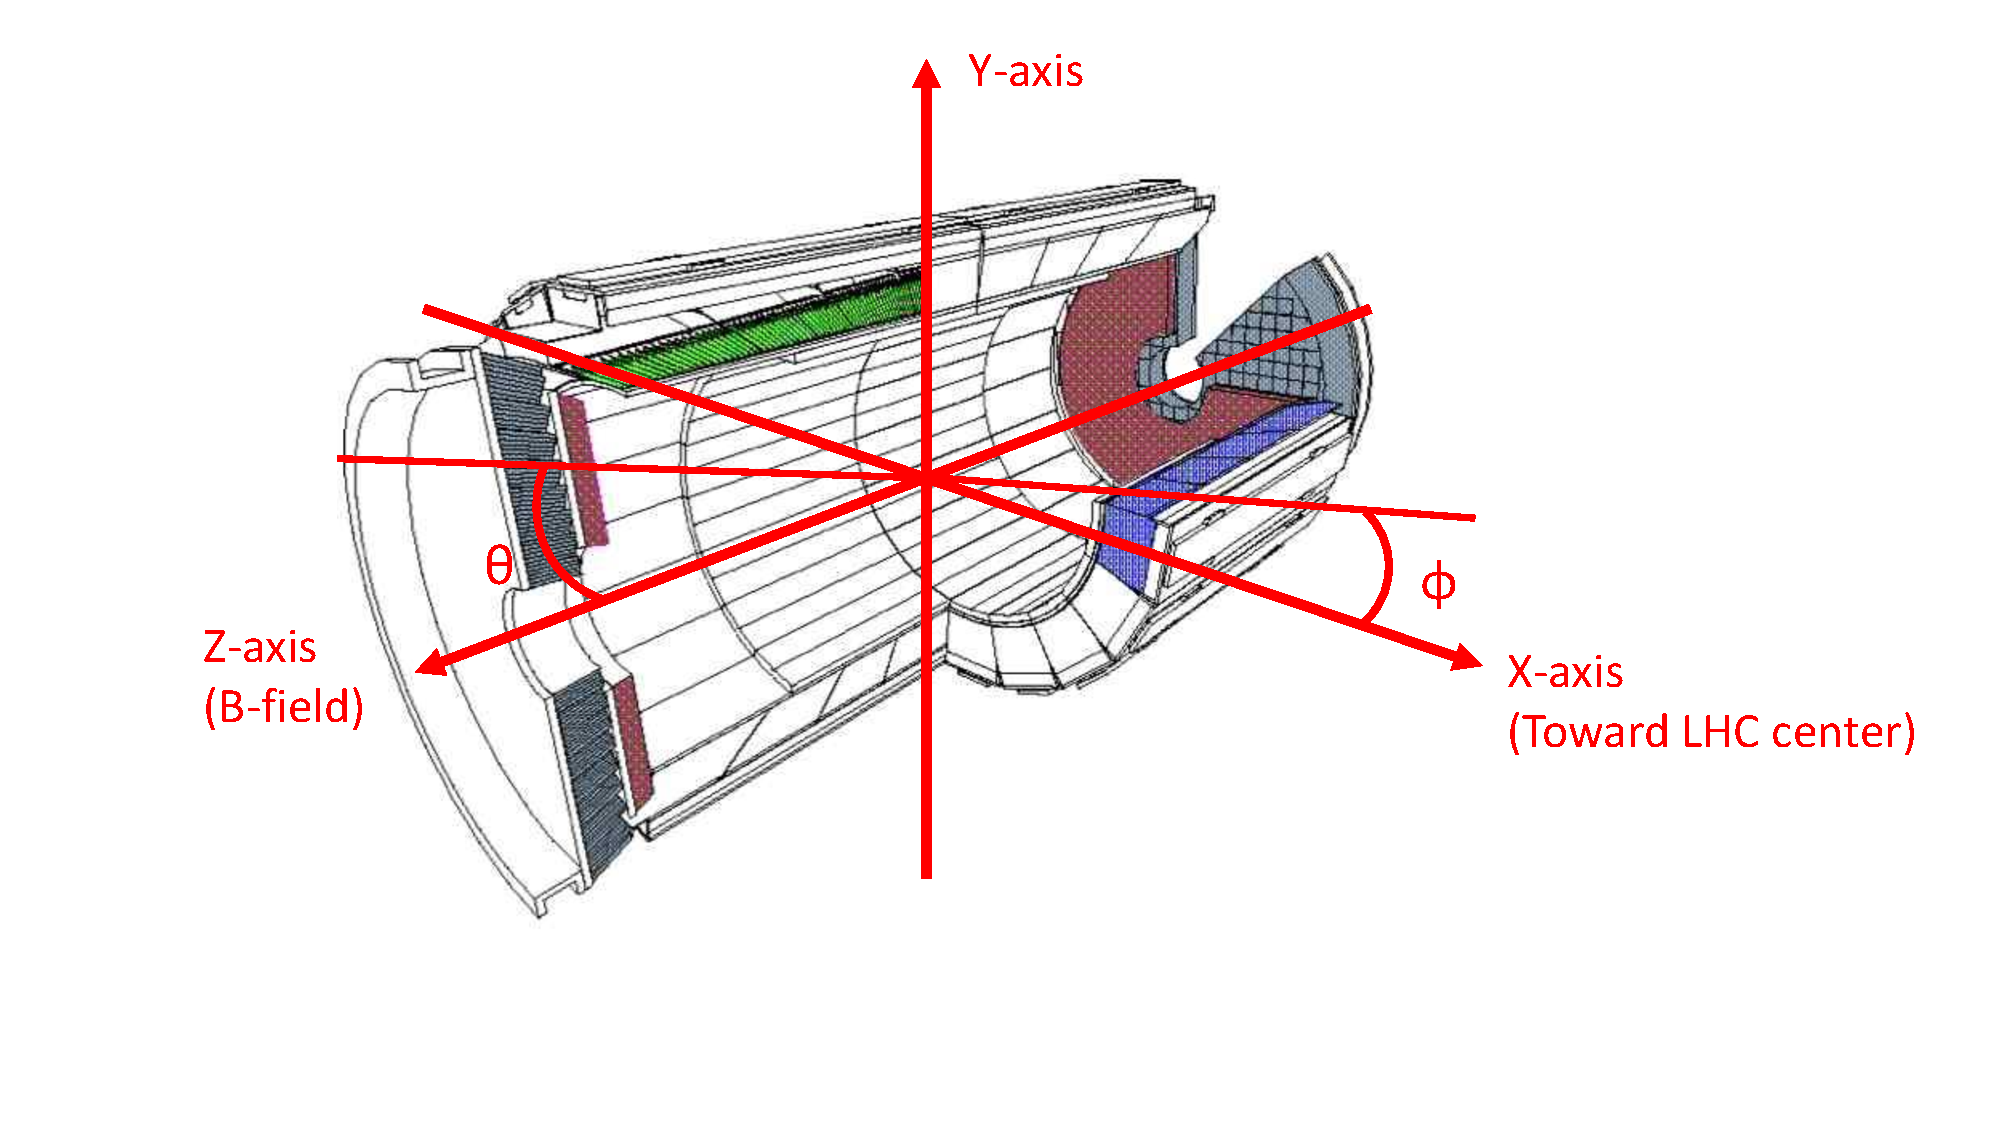
\includegraphics[width=0.95\textwidth]{Chapter2/coordinate}
	\centering
	\begin{center}
		\caption{The coordinate system used in the ATLAS detector}
		\label{Fig:coordinate}            
	\end{center}
\end{figure}
With this definition, the variation of $\eta$ is different from $\theta$, which can be seen in Fig. \ref{Fig:pseudorapidity}. This quantity is important, because the distance between two particles in the detector is defined as:
\begin{equation}
\Delta R= \sqrt{\Delta \eta^{2}+\Delta \phi^{2}}
\end{equation}
For the same $\Delta R$, the separation would be actually larger in the high $\eta$ region especially at $|\eta|>3.2$ (``endcap'' and ``forward'' regions).  
\begin{figure}[!h]                
	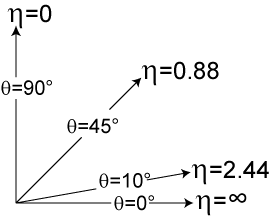
\includegraphics[width=0.4\textwidth]{Chapter2/pseudorapidity.png}
	\centering
	\begin{center}
		\caption{The Psedorapidity varied with $\theta$}
		\label{Fig:pseudorapidity}            
	\end{center}
\end{figure}

\subsection{Inner Detector (ID)}
%remember to mention MBTS
The design of a general detector usually consists of two types of system: ``trackers'' and ``calorimeters''. The tracker is used to record the particle trajectories inside the detector with the lowest disturbance on its energy, while calorimeters trap the particles to measure its total energy sum, $E$. 
\\
\\The ATLAS Inner detector is designed as a ``tracker'', so it is used to take the tracks of particles from the collisions. It stands at the inner most part of the detector and spans from 3cm to 108cm in radius with several layers from three subsystems which are pixel, semiconductor tracker (SCT) and transition radiation tracker (TRT) as shown in Fig. \ref{Fig:ID}. 

\begin{figure}[!h]                
	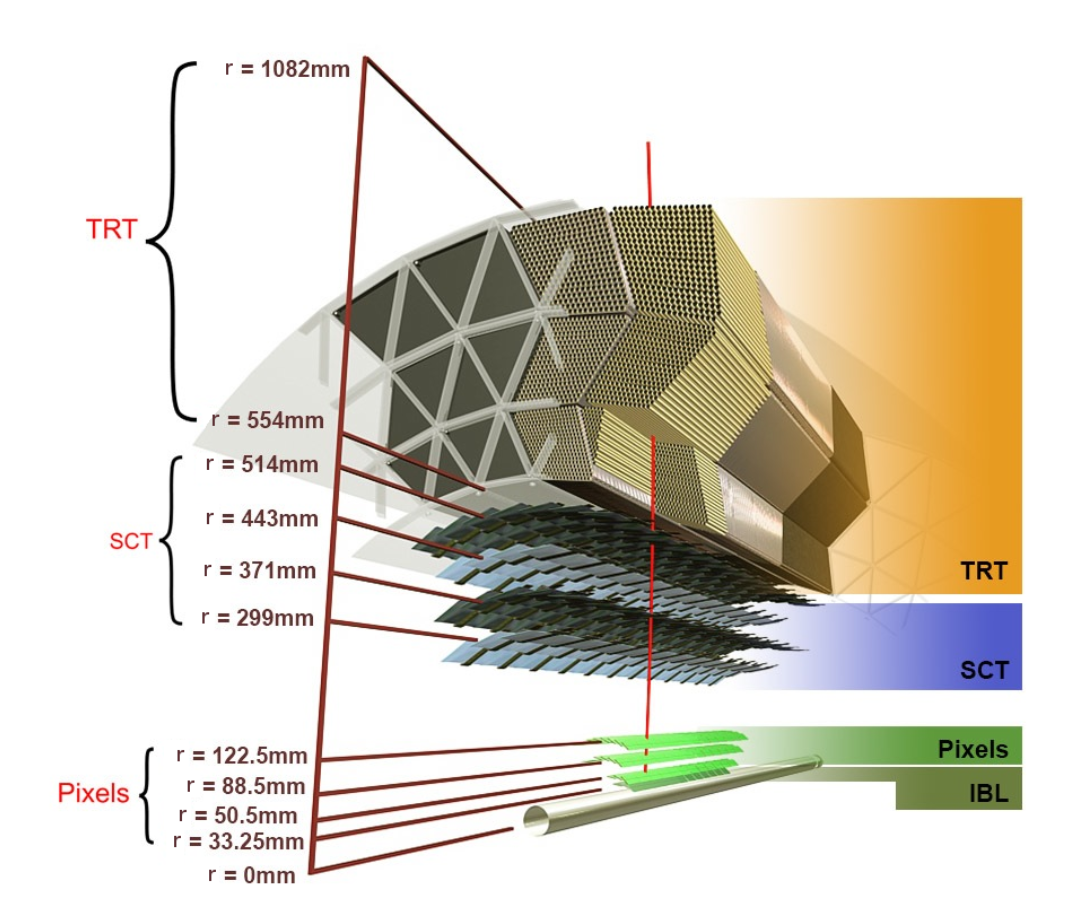
\includegraphics[width=0.7\textwidth]{Chapter2/ID.png}
	\centering
	\begin{center}
		\caption{The diagram for the ATLAS inner detector}
		\label{Fig:ID}            
	\end{center}
\end{figure}

Each layer has cells of well-defined granularity. When particles are passing through the inner detector, they leave ``a hit'' per cell on each layer. The tracks are then defined as the link through hits on each layer which are curved lines due to the existence of magnetic field from solenoid, so the curvature of a track could be taken to evaluate the particle momentum and charge. After all tracks are reconstructed, the vertexes are then defined as where the tracks cross. The resolution of transverse momentum, $p_{T}$\footnote{In ATLAS, the activity on transverse plane (i.e. x-y plan) has most of physics interest, because the transverse momentum sum is supposed to be 0, but the case for longitudinal direction isn't}, depends on the particle $p_{T}$ and $\eta$, and it can be presented as:
\begin{equation}
\sigma_{p_{T}} = \sqrt{a^{2}p_{T}^{4}+b^{2}p_{T}^{2}}
\end{equation}
with a and b, the coefficients, depending on track quality and $\eta$. From MC simulation for the track with lease seven hits (a track crossing all layers from pixel and SCT) within $0.25<|\eta|<0.5$, a and b are estimated to be 0.00034 $GeV^{-1}$ and $0.0015$ respectively.
\\
\\{\bf Pixel}
\\
\\The pixel detector is the innermost system of ATLAS, and it has the structure of three concentric barrels enclosed by three disks at each end, so all the particles coming out from the collision must pass through all the layers (giving three hits). It provides the best position resolution in the ATLAS detector with a granularity of $50\mu m\times 400\mu m$  for each cell in the $r\Delta \phi \times z$ plane with the coverage of $|\eta|<2.5$ which is used to define the barrel region which has a spatial resolution of $14\mu m\times 115\mu m$
\\
\\In 2014, a new layer of pixel detector called insertable b-layer (IBL) was installed at $3.3cm$ to the beam pipe in addition to the original three layers. Its design is aiming to assist with measurements of short-live particles (like the b quarks whose lifetime is $~10^{-12}s$), so it has an even better granularity of $50\mu m\times 250\mu m$ with extended coverage to $|\eta|<3$. The improved granularity also helps to reduce the uncertainty on impact parameter of collisions.
\\
\\{\bf Semiconductor Tracker}
\\
\\Outside the pixel detector is the semiconductor tracker with three layers in its barrel and nine disks at each end. The sensors are double sided, so when a particle passes through four layers, it leaves totally eight hits in the SCT which form four spacepoints. Different from the pixel detector which has one sensor on each module, the SCT modules have two strip sensors with the width of $80\mu m$ which cross at  an angle of $40mrad$ giving a spatial resolution of $17\mu m \times 580 \mu m$ in the $r\Delta \phi \times \Delta z$ plane. 
\\
\\{\bf Transition Radiation Tracker}
\\
\\The last part of the inner detector is the TRT detector. It doesn't have a multiple layer structure as the pixel or SCT detectors but just a single thick layer stacked of straw drift tubes. Each straw has the diameter of 4mm (with the drift time correction, the spatial resolution from each measurement is $130\mu m$) and is filled with the gas mixture of $Xe$, $CO_{2}$ and $O_{2}$. The gas mixture is used to optimize the absorption of transition radiation. (Due to the gas leaking problem found in the ATLAS operation from 2009 to 2012, part of the gas was replaced by cheaper $Ar$-based gas.) When a charge particle passes through the gas, the emitted photon (transition radiation) induces a ``charge avalanche''. This detector allows to the distinguish between electrons and charged pions (because light particles emit more transition radiation).
\\
\\{\bf Magnets}
\\
\\ The ATLAS detector has two superconducting magnet systems different from the CMS experiment with only one solenoid magnet. The inner one is the solenoid magnet located between the TRT detector and the calorimeter, while the toroid magnet is situated in the muon spectrometer system. The advantage of this design is to have the light material (solenoid) inside the detector for transparency, and the toroid still provides the magnetic field to further improve the resolution of momentum measurement.  
\\
\\The solenoid magnet is with a diameter of $2.56m$ and length of $5.8m$.  The magnetic field inside the solenoid is almost uniform of 2T along the z-axis as shown in Fig.~\ref{Fig:bfield} to give the momentum and charge measurement in the inner detector. 
\begin{figure}[!h]                
	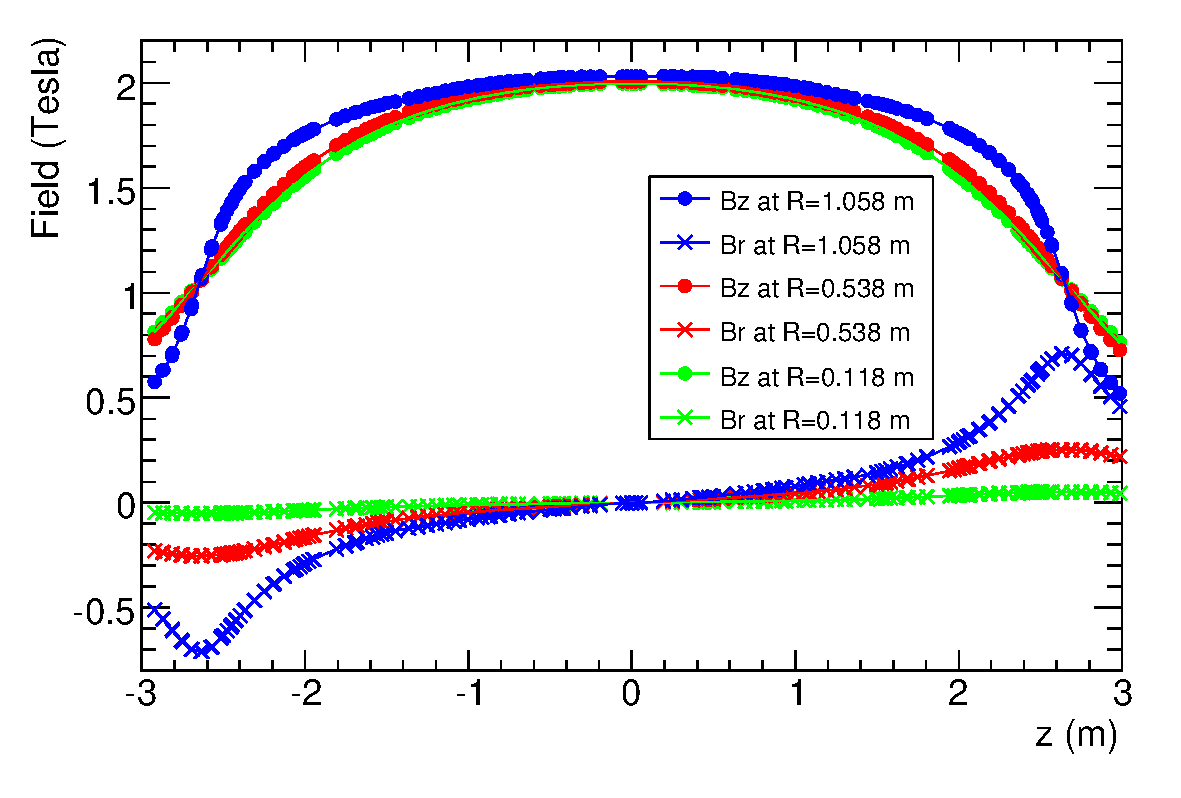
\includegraphics[width=0.6\textwidth]{Chapter2/bfield}
	\centering
	\begin{center}
		\caption{The magnetic field inside the solenoid }
		\label{Fig:bfield}            
	\end{center}
\end{figure}
\\
\\The toroid magent is composed of the barrel and endcap toroids, and both of them have eight coils providing the magnetic field of 4T in the muon spectrometer. The toroid magnet has the advantage that the particle trajectories in the transverse plane are always perpendicular to the magnetic field, so the momentum measurement is simplified. The toroid magnet is for the measurement of muon momentum in the muon spectrometer. 
\subsection{Calorimeter}
Outside the inner detector is the calorimeter, an energy sampling system. In the ATLAS analyses, there is the need to distinguish the fundamental particles with their energy, so two systems of calorimeters are applied to trap particles with different mass: the electromagnetic calorimeter (ECAL) for electrons and photons as well as the hadronic calorimeter (HCAL) for the hadronic particles. Both ECAL and HCAL have the coverage up to $|\eta|<4.9$. For the range of $|\eta|<2.5$ in the barrel region, two types of calorimeter, the liquid argon (LAr) and tile detectors, are used for the ECAL and HCAL, while in the endcap and forward regions is only the LAr detector. To fit into the cylinder shape of the ATLAS detector, the calorimeters are accordion-shaped from the cross section side. The full diagram of the calorimeter system is presented in Fig. \ref{Fig:calorimeter}. 
\begin{figure}[!h]                %
	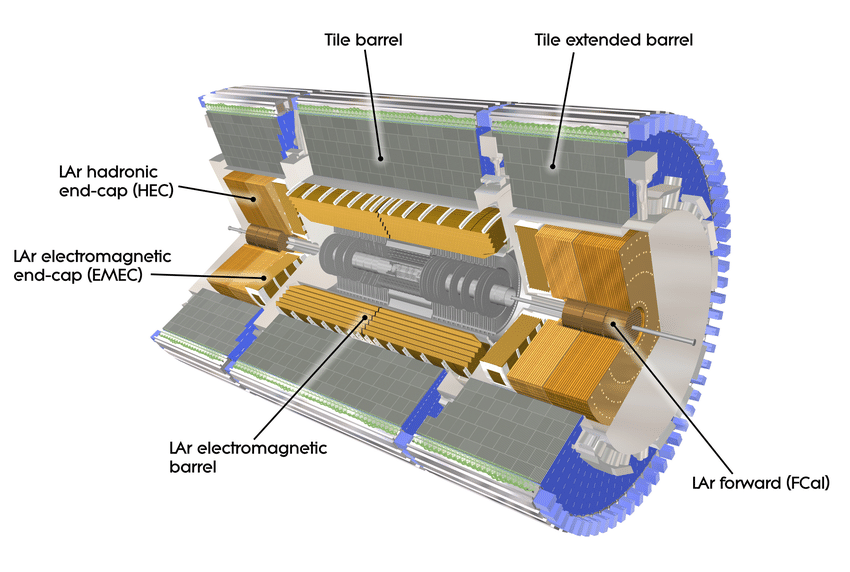
\includegraphics[width=0.85\textwidth]{Chapter2/calorimeter}
	\centering
	\begin{center}
		\caption{The calorimeter system of the ATLAS detector}
		\label{Fig:calorimeter}            
	\end{center}
\end{figure}
The energy resolution for the calorimeter could be presented as:
\begin{equation}
\sigma (E)=\sqrt{a^{2}+b^{2}E+c^{2}E^{2}}
\end{equation}
where a, b, and c are the coefficients. The first term is due to the electronic noise (constant), and the second term is from the shower development of the Poisson fluctuation for the number of shower particles, while the third terms is for the calorimeter non-uniformities (linear to the true shower energy). From the test beam data, the coefficients for the ECAL are $0.4GeV$, $0.1\sqrt{GeV}$ and $0.0017$ for a, b, and c. In terms of the HCAL, the resolution is a bit worse with $1.6GeV$, $0.52\sqrt{GeV}$ and $0.03$. The degraded resolution is due to the intrinsic property of the measurement on hadronic objects which have the energy contribution from neutrinos or binding energy between hadrons. 
\\
\\{\bf Electromagnetic Calorimeter}
\\
\\In ATLAS, the ECAL is made up of the LAr detector each module of which has one absorber and one electrode, and liquid argon is the medium between them. When a particle hits the absorber, it induces the shower, and the shower electrons ionize liquid argon atoms. All the electrons from the interactions would then be collected by the electrodes. The measured current is used to estimate the energy of the incoming particle. The process could be seen in Fig. \ref{Fig:larshower}.\\
\begin{figure}[!h]                
	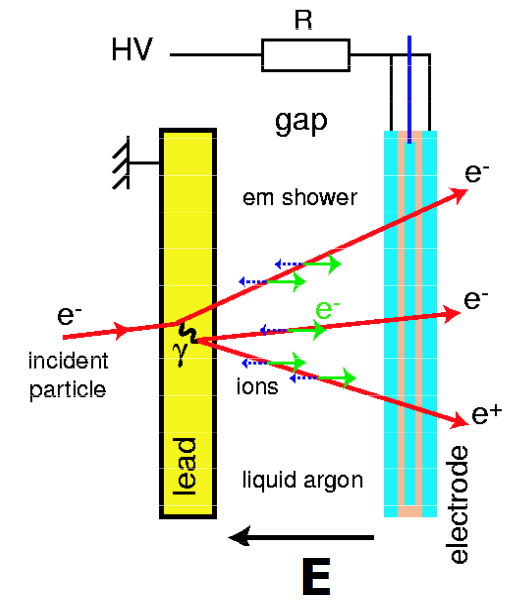
\includegraphics[width=0.35\textwidth]{Chapter2/LArshower}
	\centering
	\begin{center}
		\caption{The interaction between an electron and the LAr calorimeter}
		\label{Fig:larshower}            
	\end{center}
\end{figure}
\\The barrel LAr detector has three sampling layers with different depth and granularity. An extra presampler (layer 0) was added for $|\eta|<1.8$ which has no absorber but only a thin LAr sampler to recognize photons from $\pi^{0}$ decays. The best granularity is at the strip layer (layer 1) for $0.0031\times ~0.1$ ($\Delta \eta \times \Delta \phi$) \footnote{the granularity for $\Delta \phi$ is a approximation, as it has to complete a circle of an irrational number.}, while the last layer is coarse for $0.05 \times ~0.025$ in terms of $\Delta \eta \times \Delta \phi$. For the energy absorption, the depth is what matters most. The full depth of the three sampling layers could correspond to $\sim$22 lead radiation lengths ($X_{0}$) or 2 nuclear interaction length ($2\lambda$).\footnote{the radiation length is defined by the electron energy loss, while the nuclear interaction length is defined by the hadronic object energy loss.} When the ECAL is extended to the region of $2.5<|\eta|<3.2$, only the last two layers would remain, but they still have $18X_{0}$ in total.
\\
\\{\bf Hadronic Calorimeter}
\\
\\Behind the LAr detector is the three-layer tile detector covering $|\eta|<1.7$ with a crack\footnote{The crack is for the supporting structure and output cables} at $1.37<|\eta|<1.52$. It operates in the similar way to the LAr detector, but the absorber material is scintillator. Each sensor of this system is coarser as compared to LAr ones with $0.1 \times ~0.1$ ($\Delta \eta \times \Delta \phi$) for the first two layer and $0.1 \times 0.2$ at the third layer. With the need for the absorption of hadronic objects, it has $8 \lambda$ in the depth for all three layers.
\\
\\In the endcap region ($1.7<|\eta|<3.1$), another type of LAr detector with copper absorber is used as the HCAL. It contains four layers which have the same granularity for $0.1 \times 0.1$ ($\Delta \eta \times \Delta \phi$) in the region, $1.7<|\eta|<2.5$, and $0.2 \times 0.2$ in $2.5<|\eta|<3.1$
\\
\\{\bf Forward Calorimeter}
\\
\\In contract to the inner detector, the calorimeter should capture as many particles as possible, so the missing energy carried by invisible particles could be estimated by energy conservation within the detector. Therefore, a forward detector is installed at $3.1<|\eta|<4.9$, and it has the best rapidity coverage among the ATLAS subsystems. 
\\
\\The type of detector used here is the third type of LAr detector with tungsten absorber. It has three layers with the first one for ECAL and the last two for HCAL with the same depth of $10\lambda$ (ECAL+HCAL).  
\subsection{Muon Spectrometer}
The outermost detector is the muon spectrometer (MS). Because of their large mass and lack of strong interactions, only muons could travel through the calorimeter and leave signatures here. The muon spectrometer is composed of four types of detectors: thin gap chamber (TGC), resistive plate chamber (RPC), monitored drift tubes (MDT), and cathode strip chamber (CSC) with the toroid magnet system.  
\\
\\In this subsystem, the MDT and CSC are the two detectors providing the tracking measurement with a three-layer structure. In the coverage of $|\eta|<2.0$, all the three layers are composed of the MDT detector, while the innermost layer is replaced by the CSC detector in the extent of $2.0<|\eta|<2.7$ for the effectiveness of high particle density environment. The overall tracking measurement has the spatial resolution of $35 \mu m$
\\
\\However, the precise tracking measurement of the MDT and CSC comes with the cost of a poor temporal resolution, so the RPC ($|\eta|<1.05$) and TGC (($1.05<|\eta|<2.7$)) are interspersed in tracking layers with the time resolution of $25ns$ (with the consideration of uncertainty from cosmic muons). With the fast response, they are part of the ATLAS hardware trigger system. The overall detector performance is summarised in Tab. \ref{Tab:ms}.

\begin{table}[h]
	\caption{Muon Spectrometer Subdetector Performance}
	\renewcommand{\arraystretch}{1.3}
	\centering
	\begin{tabular}{l | c | c | c | c | c }
		\hline
		\hline
		{\bf Type}     &{\bf Function} &{\bf coverage}    &{\bf z/R resolution}  &{\bf $r \Delta \phi$ resolution}&{\bf time resolution}\\
		\hline
		MDT            &tracking       &$|\eta|<2.7$      &$35\mu m$(z)          &N/A                             &N/A            \\
		\hline
		CSC            &tracking       &$2.0<|\eta|<2.7$  &$40\mu m$(R)          &$5mm$                           &$7ns$          \\
		\hline
		RPC            &trigger        &$|\eta|<1.05$     &$10mm$(z)             &$10mm$                          &$1.5ns$         \\
		\hline
		TGC            &trigger        &$1.05<|\eta|<2.7$ &$2-6mm$(R)            &$3-7mm$                         &$4ns$           \\
		\hline
	\end{tabular}
	\label{Tab:ms}
\end{table}

\subsection{Trigger System}
The LHC has the collision rate at $~40MHz$, which leads to the data rate over $60TB$ per second. However, most of the events have no physical interest, because they are just the products of low energy hadronic interactions. Therefore, the trigger system is developed to select events which are going to the storage.
\\
\\For data-taking, the ATLAS trigger system has a two-level structure: the hardware-based L1 trigger (L1) and the software-based high level trigger (HLT). The L1 system is based on the front-end electronics with the logic of selection written by FGPA. Its feature is to make a fast reconstruction of physical objects with a degraded resolution, and it delivers the events at the rate of $100kHz$ ($100k$ events per second). As the detector signatures from the calorimeter and MS are irrelevant to each other, they have their independent L1 trigger systems: L1Calo and L1MU. After the physical objects objects are reconstructed in the two systems, they are then sent to the L1Topo system for the estimation on the topological relation between them. The final trigger decision would eventually be made at the central trigger processor (CTP) by whether a event contains the objects with energy or topological parameters fulfilling the defined criteria. Afterwards, those objects are further processed with a more complicated reconstruction algorithm to give the HLT trigger decision, and the output event rate is reduced to $\sim 1kHz$. The full trigger system is shown in Fig. \ref{Fig:trigger}.
\begin{figure}[!h]                
	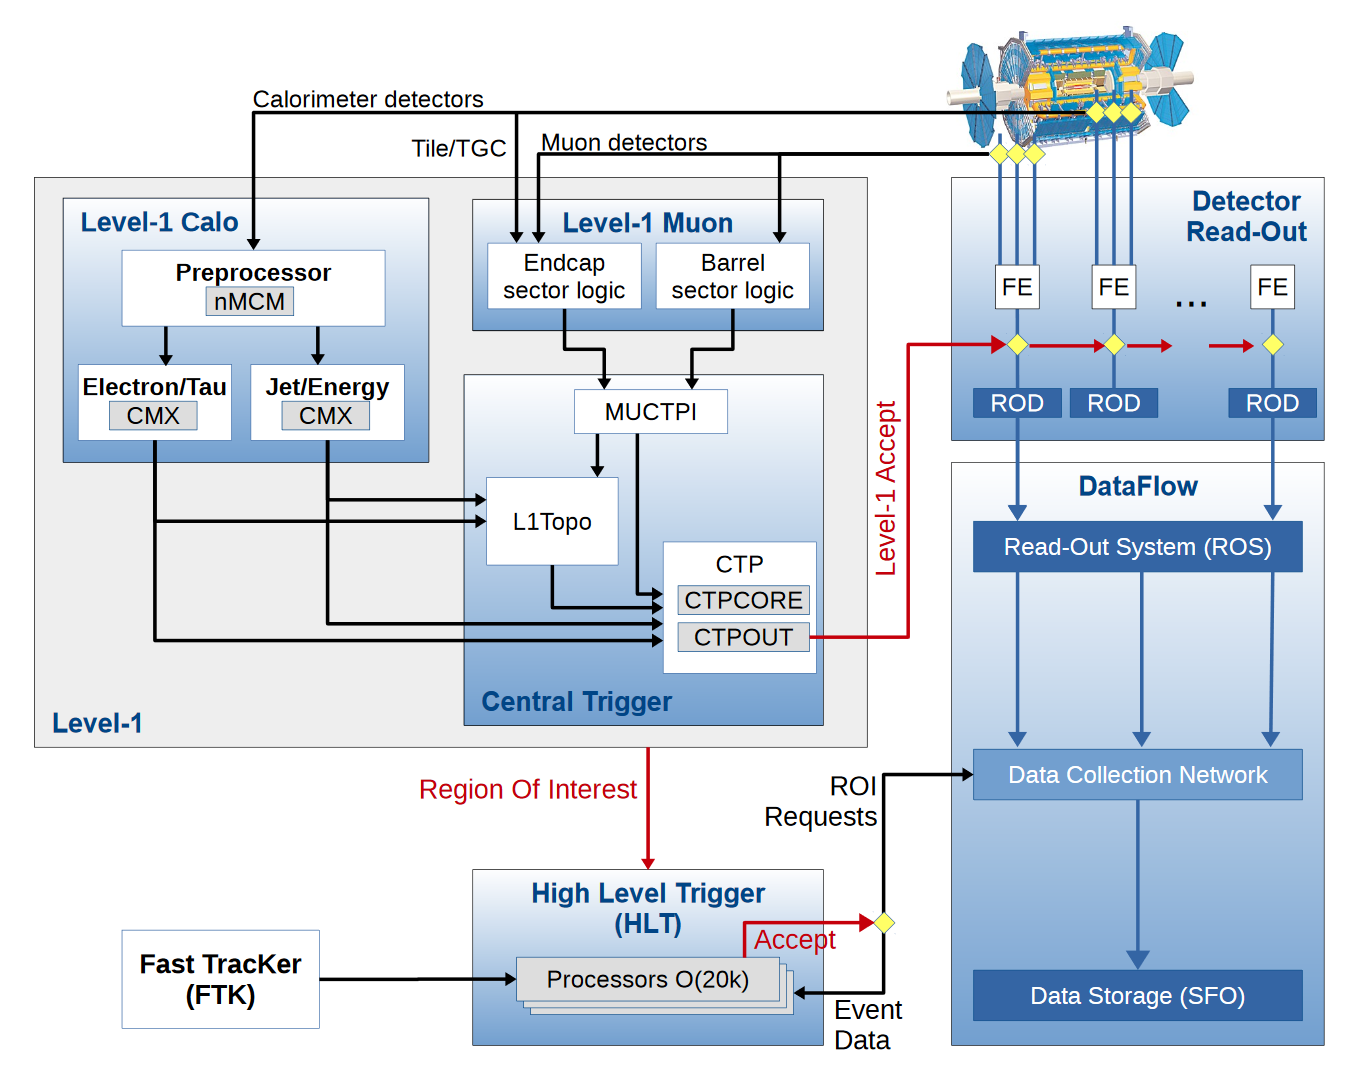
\includegraphics[width=0.8\textwidth]{Chapter2/Trigger.png}
	\centering
	\begin{center}
		\caption{The ATLAS trigger system}
		\label{Fig:trigger}            
	\end{center}
\end{figure}
\noindent
\\{\bf L1Calo}
\\
\\When the detector signatures are received from the calorimeter, they are firstly sent to the readout buffer and the L1Calo sysetm. The first component in the L1Calo electronic system is the preprocessor where the signatures are processed into trigger towers with degraded granularity and sent to the processors for physical object reconstruction. Electrons, photons and taus are reconstructed with the trigger tower of $0.1 \times 0.1 (\Delta \eta \times \Delta \phi)$ in the cluster processor (CP), while hadronic objects and missing transverse energy ($E_{T}^{missing}$)\footnote{As the protons only have the longitudinal momentum, the transverse direction momentum should be conserved after collisions} are processed in jet energy processor (JEP) with a coarser granularity of $0.2\times 0.2$.
\\
\\{\bf L1MU}
\\
\\The L1MU system is taking the data from the RPC and CSC which have great time resolution as fast as $1.5\mu s$ but with a poor spatial resolution. It receives signatures from the MS barrel and endcaps where they are processed respectively. To further suppress the rate contributed by fake muons, the L1 muons are reconstructed with consistent hits from the TGC at the endcap ($1.05<|\eta|<2.7$). 
\\
\\{\bf HLT}
\\
\\When the trigger decision was made to accept an event, the regions of interest (ROI) with the original detector granularity are passed to the HLT. The HLT is runs on a CPU farm where the more complicated algorithms are deployed to reconstruct the physical objects. Due to the finer granularity and longer latency, it provides better precision on both energy and spatial resolution. When the events fulfil the HLT criteria, they are then sent to storage. 
\\
\\{\bf ATLAS Trigger Menu}
\\
\\An ATLAS trigger is generally a trigger chain composed of L1 and HLT items. When an HLT trigger is fired, there is always a corresponding L1 trigger decision. For example, HLT electron trigger shall only be passed when a L1 electron trigger is also fired:
\begin{equation}
L1\_e24 \rightarrow HLT\_e26\_lhtight\_nod0\_ivarloose
\end{equation}
where the numbers are the trigger thresholds in the unit of $GeV$, while the $lhtight$ and $ivarloose$ are to define the electron quality with the calorimeter activities in the surrounding region of this electron (see more details in Sec. \ref{sec:obj rec}) . The threshold of triggers might not be kept the same during the operation at periods. Because the LHC keeps pushing its performance on instantaneous luminosity, the energy contribution from pile-up events enhances the trigger rate above the allowed bandwidth for data storage. To make better suppression on the trigger rate, the thresholds are therefore raised during some operation periods. 
\\
\\The defined triggers would then be made into ``streams'' where the events are categorized for different purposes. Physics analyses shall use the triggers contained in the ``$physics\_main$'' stream, and there are also the dedicated streams composed of ``prescaled'' triggers for hardware calibrations. Those calibration triggers usually have lower thresholds in contract with the ones in $physics\_main$. A random sampling is applied to only pick a fraction of events passing those triggers, which makes them unsuitable for physics analysis. The total allowed output rate from all streams is $5kHz$ with $1kHz$ for $physics\_main$. 

\subsection{Run 2 Operation Overview}
For the ATLAS operation from 2015 to 2018 which is called Run 2 (with respect to Run 1 from 2009 to 2013), the average data recording efficiency is around $95\%$ with respect to LHC delivery efficiency. The integrated luminosity is $\sim~36fb^{-1}$ for 2015 and 2016, $\sim46~fb^{-1}$ for 2017 and $\sim63~fb^{-1}$ for 2018 which gives the total data of $140 fb^{-1}$. The performance from 2011 to 2018 is summarized in Fig. \ref{Fig:recefficiency}


